% !TEX encoding = UTF-8 Unicode
%!TEX TS-program = xelatex

\documentclass[12pt]{extarticle}
% extarticle is like article but can handle 8pt, 9pt, 10pt, 11pt, 12pt, 14pt, 17pt, and 20pt text

\def \ititle {Origins of Mind}
 
\def \isubtitle {Lecture 08}
 
\def \iauthor {Stephen A. Butterfill}
\def \iemail{s.butterfill@warwick.ac.uk}
\date{}

%for strikethrough
\usepackage[normalem]{ulem}

\input{$HOME/Documents/submissions/preamble_steve_handout}

%logic symbol \leftmodels
\usepackage{MnSymbol}

%\bibpunct{}{}{,}{s}{}{,}  %use superscript TICS style bib
%remove hanging indent for TICS style bib
%TODO doesnt work
\setlength{\bibhang}{0em}
%\setlength{\bibsep}{0.5em}


%itemize bullet should be dash
\renewcommand{\labelitemi}{$-$}

\begin{document}

%\raggedcolumns

\begin{multicols*}{3}

\setlength\footnotesep{1em}


\bibliographystyle{newapa} %apalike

%\maketitle
%\tableofcontents




%--------------- 
%--- start paste


\def \ititle {Logic I}
 
\def \isubtitle {Lecture 07}
 
\begin{center}
 
{\Large
 
\textbf{\ititle}: \isubtitle
 
}
 
 
 
\iemail %
 
\end{center}
 
Readings refer to sections of the course textbook, \emph{Language, Proof and Logic}.
 
 
 
\section{The Syntax of FOL}
 
\emph{Reading:} §9.3
 
We define what counts as a sentence of FOL using rules. E.g.:
 
1. If * and \# are sentences, then so is(* ∧ \#)
 
2. If * and \# are sentences, then so is (* ∨ \#)
 
3. P, Q, R, … are sentences
 
4. If * is a sentence, then ¬* is a sentence
 
So:
 
a. P is a sentence // rule 3
 
b. ¬P is a sentence // rule 4, a
 
c. ( ¬P ∧ Q ) is a sentence // rule 1, b, a
 
There is no structural ambiguity in FOL because these rules are formulated to ensure that for any FOL sentence, there is exactly one way of constructing it.
 
\begin{center}
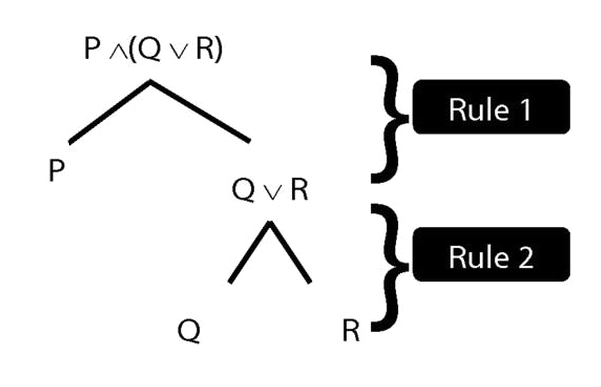
\includegraphics[scale=0.3]{img/unit_230_tree1.png}
\end{center}
\begin{center}
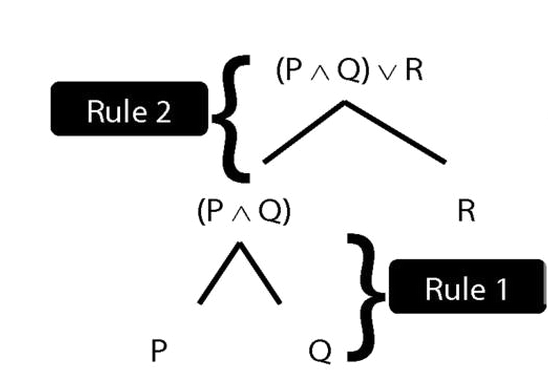
\includegraphics[scale=0.3]{img/unit_230_tree2.png}
\end{center}
\begin{center}
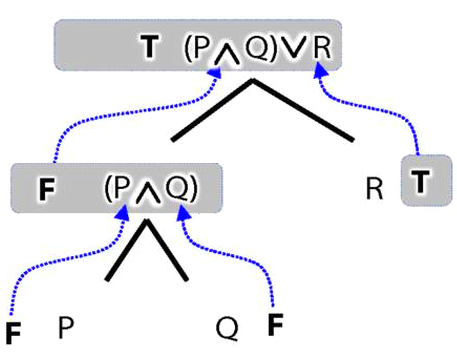
\includegraphics[scale=0.3]{img/unit_230_tree_tt.png}
\end{center}
 
 
\section{¬P ∨ ¬Q compared with ¬(P ∨ Q)}
 
\emph{Reading:} §3.5
 
 
 
\section{Subproofs Are Tricky: The Answer}
 
\begin{center}
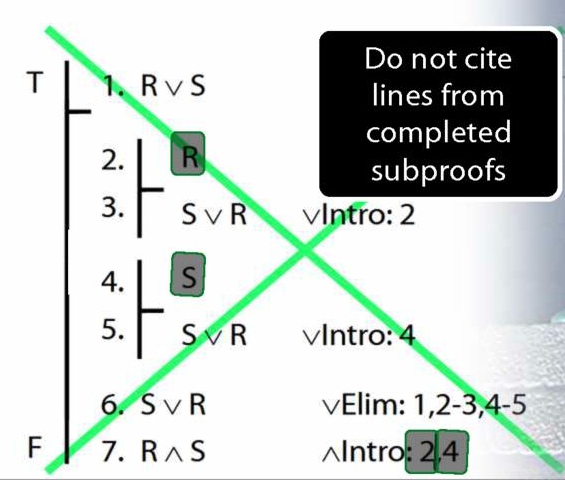
\includegraphics[scale=0.3]{img/unit_227_tricky_answer.png}
\end{center}
 
 
\section{¬Intro Proof Example}
 
\emph{Reading:} §5.3, §6.3
 
\begin{center}
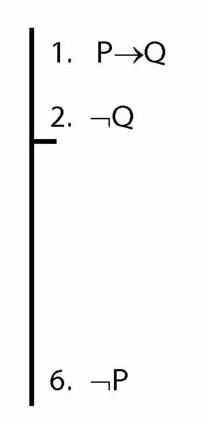
\includegraphics[scale=0.3]{img/unit_283_proof.png}
\end{center}
 
\begin{minipage}{\columnwidth} 
\section{DeMorgan: ¬(A ∧ B) $\leftmodels\models$ ¬A ∨ ¬B}
 
\emph{Reading:} §3.6, §4.2
 
`$\leftmodels\models$' means `is logically equivalent to', so for now `has the same truth table as'.
 
A $\leftmodels\models$ ¬¬A
 
¬(A ∧ B) $\leftmodels\models$ (¬A ∨ ¬B)
 
¬(A ∨ B) $\leftmodels\models$ (¬A ∧ ¬B)
 
A → B $\leftmodels\models$ ¬A ∨ B
 
¬(A → B) $\leftmodels\models$ ¬(¬A ∨ B) $\leftmodels\models$ A ∧ ¬B
 
\end{minipage} 
 
\section{Everything Is Broken}
 
\emph{Reading:} §9.1, §9.2
 
Everything is broken: ∀x Broken(x)
 
Something is broken: ∃x Broken(x)
 
\vfill
\begin{minipage}{\columnwidth}
\section{Exercises}
These exercises will be discussed in seminars the week after this lecture.
The numbers below refer to the numbered exercises in the course textbook, e.g.\ `1.1' refers to exercise 1.1. on page 39 of the second edition of \emph{Language, Proof and Logic}.
 
\begin{quote}
6.24--6.26
 
3.19
 
4.15--18
 
9.1 odd numbers only
 
9.2 even numbers only
 
\end{quote}
\end{minipage}
%--- end paste
%--------------- 
 


\end{multicols*}

\end{document}